\problemname{\problemyamlname}

%\illustration{0.3}{image.jpg}{Caption of the illustration (optional). CC BY-NC 2.0 by X on Y}
% Source: URL to image.

% optionally define variables/limits for this problem

Jérôme and his two teammates must get to KARWa at UMons.
Unfortunately, they made a mistake and ended up at UCLouvain!
They don't have much time and so ask their friend Nicolas - an expert of maps and of shortest parts - who has a map with $n$ stations and $m$ bidirectional train lines each taking some time $w$.
Can you determine if they'll arrive in time?

UCLouvain is represented by the $1$ intersection and UMons by the $n$ intersection.
A path is guaranteed between the two universities.

\begin{figure}[h]
	\centering
	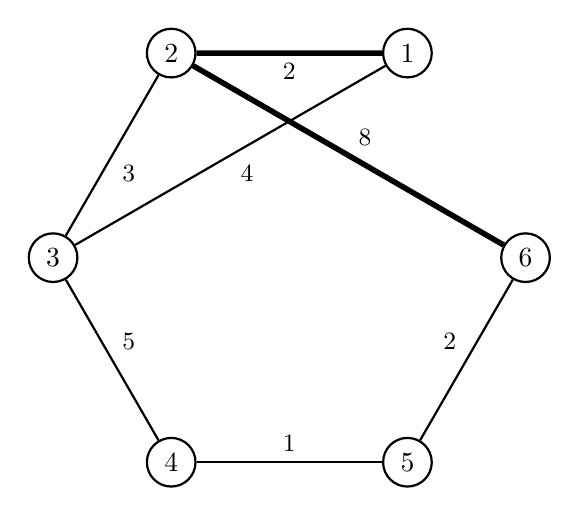
\begin{tikzpicture}[auto,node distance=2cm,thick]
		\tikzset{edge/.style = {draw, -}}
		\tikzset{weight/.style = {font=\small}}
		
		% nodes
		\foreach \i in {1,...,6}
			\node[circle,draw] (\i) at (360/6*\i:3) {\i};
		
		% edges and weights
		\draw[edge] (1) -- node[weight]{2} (2);
		\draw[edge] (1) -- node[weight]{4} (3);
		\draw[edge] (2) -- node[weight]{3} (3);
		\draw[edge] (2) -- node[weight]{8} (6);
		\draw[edge] (3) -- node[weight]{5} (4);
		\draw[edge] (4) -- node[weight]{1} (5);
		\draw[edge] (5) -- node[weight]{2} (6);
		
		% path from 1 to 6 in bold
		\draw[line width=2pt] (1) -- (2) -- (6);
		
		% uncomment the following line to add labels to the nodes
		% \foreach \i in {1,...,6} \node at (360/6*\i:3.5) {\i};
		\end{tikzpicture}
		
\caption[short]{Example 1: the path from 1 to 6 is bold}
\end{figure}
	

\begin{Input}
	The input consists of :
	\begin{itemize}
		\item One line with two integers $n$ and $m$ ($2 \le n, m \le 10^6$), where $n$ is the number of intersections and $m$ is the number of connections,
		\item $m$ lines with 3 integers each $u$ ($1 \le u \le n$), $v$ ($1 \le v \le n$), and $w$ ($1 \le w \le 10^6$), which represent a bidirectional connection between $u$ and $v$, with a time of $w$.
	\end{itemize}
\end{Input}

\begin{Output}
	An integer with the length of the shortest path between $1$ and $n$.
\end{Output}
